
%%% Definição de problema multi-objectivo

Na vida real é comum a existência de problemas de otimização que
consideram mais de um objetivo os quais, geralmente, são conflitantes.
Estes problemas são chamados multiobjetivos e tipicamente não possuem
solução ótima, ou seja, uma solução que é a melhor em todos os objetivos,
mas as soluções de interesse as chamadas \emph{soluções eficientes}.

Um problema de otimização multi-objetivo com $\np$ objetivos pode ser descrito como uma
função vetorial $f(x) = \big(f_1(x), \ldots, f_p(x)\big)$
para a qual deseja-se encontrar um vetor $x \in X$
que maximize simultaneamente as $\np$ funções objetivo.
Formalmente:
\begin{align*}
  \text{max} ~ f(x) &=
    \big(f_1(x)
    ,f_2(x)
    ,\ldots
    ,f_{\np}(x)\big) \\
  \text{sujeito a} ~ x & \in X
\end{align*}

Considere um problema de otimização multi-objetivo.
Diz-se que uma solução $x \in X$
\emph{domina} uma solução $y \in X$, denotado por $\text{dom}(x, y)$
se, e somente se, $x$ é ao menos tão boa quanto
$y$ em todos os objetivos e melhor que $y$ em ao menos um dos objetivos.
Formalmente:
\begin{displaymath}
    \text{dom}(x, y) = \left\{
      \begin{array}{l}
          \forall i \in \{1, 2, \ldots, \np\}: f_i(x) \geq f_i(y) ~\text{e}\\
          \exists j \in \{1, 2, \ldots, \np\}: f_j(x) > f_j(y)
  \end{array} \right.
\end{displaymath}
Uma solução $x \in X$ é dita \emph{eficiente}, denotado por $\text{eff}(x)$,
se, e somente se, $x$ não é dominada por nenhuma outra solução pertencente a $X$.
O conjunto de todas as soluções eficientes de um problema multi-objetivo,
denotado por $Par(X)$, é chamado de \emph{\paretoset{}} ou \emph{\paretosetII{}}.
Formalmente:
\begin{displaymath}
  Par(X) = \{ x \in X \;|\; \text{eff}(x)\}
\end{displaymath}
O conjunto de todas as soluções eficientes de um problema multi-objetivo
é chamado de \emph{\paretoset}.
Resolver um problema multi-objetivo consiste em determinar seu \paretoset{}.
Este conceito foi primeiramente elaborado por Vilfredo Pareto em 1896, que
enunciou a relação Pareto-Ótima que diz: ``não é possível melhorar uma característica
do problema sem piorar outra'', o que caracteriza a relação conflitante entre os
objetivos na otimização multi-objetivo.
%% Comentar sobre a dificuldade dos problemas multi-obj (numero de objetivos)

%%% Intro ao MOKP

Um dos problemas multiobjetivos mais importantes da literatura
é o problema da mochila multiobjetivo (\mokp{}).
Muitas problemas reais podem ser modelados como uma instância do \mokp{}
como seleção de projetos~\cite{teng1996multiobjective},
orçamento de capital~\cite{rosenblatt1989generating},
carregamento de carga~\cite{teng1996multiobjective}
e planejamento de estoque~\cite{ishibuchi2015behavior}.

%%% Definição do MOKP

O problema da mochila multi-objetivo pode ser descrito como uma função vetorial
$f$ que mapeia uma variável de decisão (solução) a uma tupla de $\np$ valores
(objetivos).
Formalmente:
\begin{align*}
  \text{max} ~ \sol{y} &= f(\sol{x}) =
    \big(f_1(\sol{x})
    ,f_2(\sol{x})
    ,\ldots
    ,f_{\np}(\sol{x})\big) \\
  \text{sujeito a} ~ \sol{x} & \in X
\end{align*}
onde $\sol{x}$ é a \emph{variável de decisão}, $X$ denota o conjunto de
soluções viáveis e $\sol{y}$ representa o \emph{vetor de objetivos} para os quais
deseja-se maximizar.


Vale resaltar que o tamanho do \paretoset para o problema em questão
tende a crescer rapidamente com o tamanho do problema, especialmente com o
número de objetivos.

Uma instância de um problema da mochila multi-objetivo (\mokp{}) com $\np$
objetivos consiste em uma capacidade inteira $W >0$ e $n$ itens.
Cada item $i$ possui um peso inteiro positivo $w_i$ e $\np$ lucros inteiros
$p_i^1, p_i^2, \ldots, p_{i}^{\np}$ não negativos.
O lucro $p_i^k$ representa a contribuição do $i$-ésimo item
para com o $k$-ésimo objetivo.
Uma solução é representada por um conjunto $\sol{x} \subseteq \{1, \ldots, n\}$
contendo os índices dos itens incluídos na mochila.
Uma solução é viável se o peso total incluído na mochila não ultrapassa
a capacidade da mochila.
Formalmente a definição do problema é a seguinte:
\begin{align*}
  \text{max   } & f(\sol{x}) =
    \big(f_1(\sol{x}) ,f_2(\sol{x}) ,\ldots ,f_{\np}(\sol{x})\big) \\
  \text{subject to   } & w(\sol{x}) \leq W \\
  & \sol{x} \subseteq \setIN\\
  \text{where} \phantom{mmmmm} \\
  %I_n &= \{1, \ldots, n\}\\
  f_j(\sol{x}) &= \sum_{i \in \sol{x}} p^j_i \quad j = 1, \ldots, m\\
  w(\sol{x}) &= \sum_{i \in \sol{x}} w_i
\end{align*}


O \mokp{} é considerado um problema \nphard{} visto set uma generalização
do bem conhecido problema da mochila $0-1$, para o qual $\np = 1$.
É consideravelmente difícil determinar o \paretoset para um \mokp{},
especialmente para vários objetivos.
Até mesmo para casos bi-objetivos, problemas pequenos podem se apresentar
intratáveis.
Por este motivo interessa-se no desenvolvimento de métodos eficientes
para manipular uma grande quantidade de soluções, o que pode eventualmente
trazer tratabilidade a instâncias antes intratáveis.

Considerando duas soluções $\sol{x}, \sol{y} \subseteq \setIN$,
$\sol{y}$ é considerada \emph{extensão} de $\sol{x}$, denotada como $\ext{y}{x}$,
se, e somente se, $sol{x} \subseteq \sol{y}$.
Qualquer conjunto $\sol{e} \subseteq \setIN$ tal que $\sol{x} \cap \sol{e} = \emptyset$
é dito ser um \emph{extensor} de $\sol{x}$.
Se $\weight{x} + \weight{e} \leq W$ então $\sol{e}$ é considerado um
\emph{extensor viável} de $\sol{x}$.
Uma solução $\sol{x}$ é chamada \emph{deficiente} se esta ainda possui capacidade
suficiente para incluir um ou mais itens, ou seja, $\weight{x} + min\{ w_i : i \notin \sol{x} \} \leq W$.
Considera-se que $\sol{x}$ \emph{\knapsackdominates} $\sol{y}$, denotado por
$\domk{x}{y}$, se $\sol{x}$ domina $\sol{y}$ e não pesa mais que $\sol{y}$.
Formalmente:
\begin{equation}
  \label{eq:kdom}
  \domk{x}{y} = \left\{
    \begin{array}{l}
      \dom{x}{y} \quad \text{and} \\
      w(\sol{x}) \leq w(\sol{y})
    \end{array}
  \right.
\end{equation}

O conceito de dominância segundo a mochila foi primeiramente proposto por
Weingartner e Ness~\cite{weingartner1967methods}.

A Figura~\ref{fig:kdom} ilustra o conceito para um problema com $\np = 1$.
Qualquer solução na área hachurada domina segundo a mochila a solução assinalada.
Este conceito é largamente utilizado em diversos algoritmo, inclusive no
algoritmo exato abordado neste Capítulo.

\begin{figure}
  \centering
  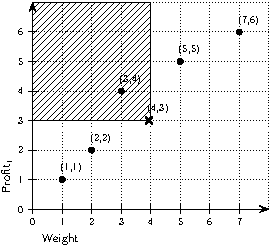
\includegraphics[scale=1.2]{img/kdt/dom}
  \caption{A knapsack-dominated solution.}
  \label{fig:kdom}
\end{figure}

A literatura contém várias propostas para resolver o \mokp{} de forma exata.
Porém, nenhum método tem provado ser eficiente para grande instâncias
com mais de dois objetivos.
Mesmo para problemas bi-objetivo, algumas instâncias de tamanho considerado
médio têm aprestando difculdades na determinação da solução exata, o que
tem motivado o desenvolvimento de métodos heurísticas que buscam determinar
um \paretoset aproximado em tempo computacional razoável.
